\subsection{Теоритическая основа}

\qquad Frequency Shift Key - вид модуляции, при которой скачкообразно изменяется частота несущего сигнала в зависимости от значений символов информационной последовательности. Частотная модуляция весьма помехоустойчива, так как помехи искажают в основном амплитуду, а не частоту сигнала.
\quad Для начала рассмотрим двоичную FSK модуляцию, когда исходный модулирующий сигнал  представляет собой двоичную бинарную последовательность нулей и единиц следующую с битовой скоростью
    
    \begin{figure}[H]
	\begin{center}
		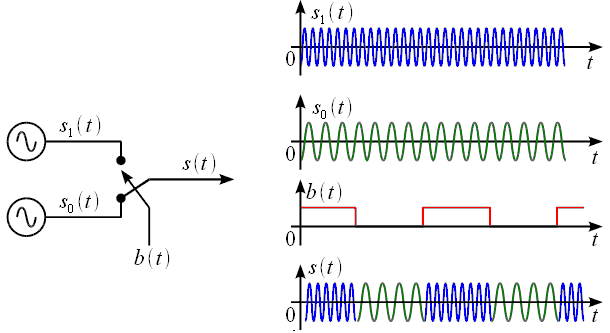
\includegraphics[scale=0.4]{fig/lab12/fsk.png}
		\caption{Пример FSK с двоичными данными}
		\label{pic:fsk_example} % название для ссылок внутри кода
	\end{center}
\end{figure}

\quad Частотно-манипулированные FSK сигналы одни из самых распространенных в современной цифровой связи. Это обусловлено прежде всего простотой их генерирования и приема, ввиду нечувствительности к начальной фазе. В данной статье мы рассмотрим принцип формирования и параметры FSK модуляции и одной из ее модификаций — CPFSK (FSK с непрерывной фазой).

\subsection{Схема в GNU Radio}    
    Для изучения этого процесса в GNU Radio\cite{gnuradio} необходимо построить следующую блок схему \ref{pic:fsk_scheme}:
    
    \begin{landscape}
	\begin{figure}[H]
		\centering
		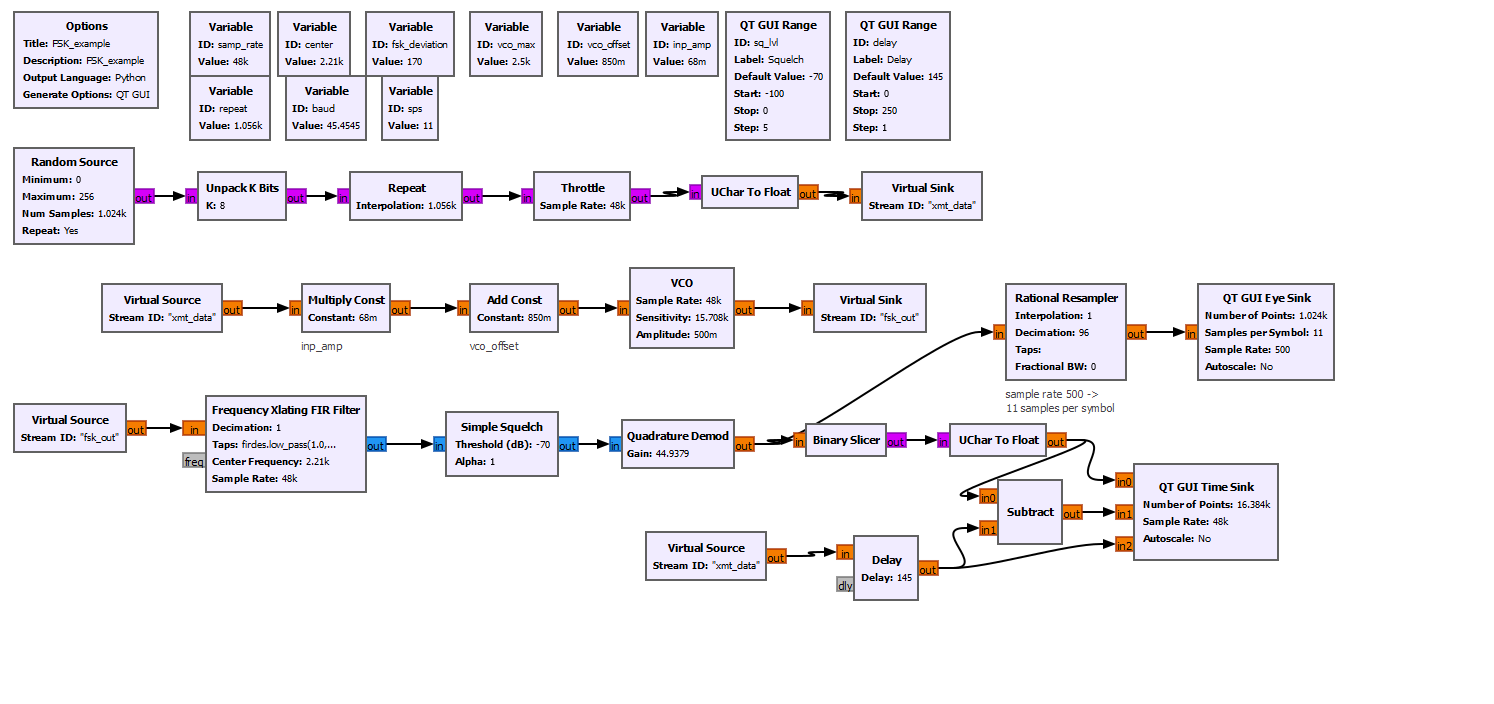
\includegraphics[width=25.5cm]{fig/lab12/fsk_scheme.png}
		\caption{Схема FSK}
		\label{pic:fsk_scheme} % название для ссылок внутри кода
	\end{figure}
\end{landscape}

Для лучшего понимания опишем используемые блоки:
\begin{itemize}
	\item Variable - блок адресующий в уникальной переменной. При помощи ID можно передавать информацию через другие блоки.
	\item QT GUI Range - графический интерфейс для изменения заднной переменной.
	\item Random Source - генератор случайных чисел.
	\item Unpack K bits - преобразуем байт с k релевантными битами в k выходных байтов по одному биту в каждом.
	\item Repeat - количество повторенний ввода, деуйствующее как коэффицент интерполяции.
	\item Throttle - дросселировать поток таким образом, чтобы средняя скорость не превышала удельную скорость.
	\item Uchar To Float - конвертация байта в Float.
	\item Virtual Sink - сохраняет поток в вектор, что полезно, если нам нунжо иметь данные за эксперимент.
	\item Virtual Source - источник данных, который передаёт элементы на основе входного вектора.
	\item Multiply Const - умножает входной поток на скаляр или вектор.
	\item Add Const - прибавляет к потоку скаляр или вектор.
	\item VCO - генератор, управляемый напрямжением. Создает синусойду на основе входной ампилтуды.
	\item Frequency Xlating FIR Filter - этот блок выполняет преобразование частоты сигнала, а также понижает дискретизацию сигнала, запуская на нем прореживающий КИХ-фильтр. Его можно использовать в качестве канализатора для выделения узкополосной части широкополосного сигнала без центрирования этой узкополосной части по частоте. 
	\item Simple Squelch - простой блок шумоподавления на основе средней мощности сигнала и порога в дБ.
	\item Quadrature Demod - квадратурная модуляция.
	\item Binary Slicer - слайсы от значения с плавающей запятой, производя 1-битный вывод. Положительный ввод производит двоичную 1, а отрицательный ввод производит двоичный ноль. 
	\item QT GUI Sink - выводы необходимой инфомрации в графическом интерфейсе.
\end{itemize}

В этом примере используется Baudot Radioteletype, следовательно битовое время = 22 миллисекунды. Получаем скорость передачи 45,4545.
Коэффицент повторения равен samp\_rate * 0,022.

В VCO генерируются сигналы 2295 Гц (отметка = 1) и 2125 Гц (отметка = 0). При выборе полной шкалы частоты 2500 Гц (vco\_max) для входа +1 чувствительность VCO = (2 * math.pi * 2500 / 1) = 15708. Можно использовать любую частоту выше 2295 Гц. 2500 Гц — хорошее круглое число. Глядя на вывод виртуального источника «xmt\_data», Mark = +1.0 и Space = 0.0. Частота отметки 2295 Гц создается вектором inp\_amp = (1,0 * 0,068) + vco\_offset = 0,918, что равно (2295/2500). Параметр отводов частотного Xlating FIR Filter равен 'firdes.low\_pass(1.0,samp\_rate,1000,400)'.

Теперь посмотрим, что у нас с данными:

Источник:
генерирует случайные байты (от 0 до 255). Далее этот байт распоковывается в каждый бит становится байтом со значащим младшим разрядом. Для ограничения потока использует Throttle.

Приёмник:
при помощи фильтра смещает принимаемый сигнал так, чтобы он был сосредоточен вокруг центральной частоты - между частотами Mark и Space. Шумоподавитель добавлен для реального приёма сигналов. Блок Quadrature Demod производит сигнал, который является положительным для входных частот выше нуля и отрицательным для частот ниже нуля. Когда данные доходят до Binary Slicer, то на выходе получает биты, это и есть наша полученная информация.
\subsection{Тестирование}
Запустим моделирование и посмотрим что имеем.

    \begin{figure}[H]
	\begin{center}
		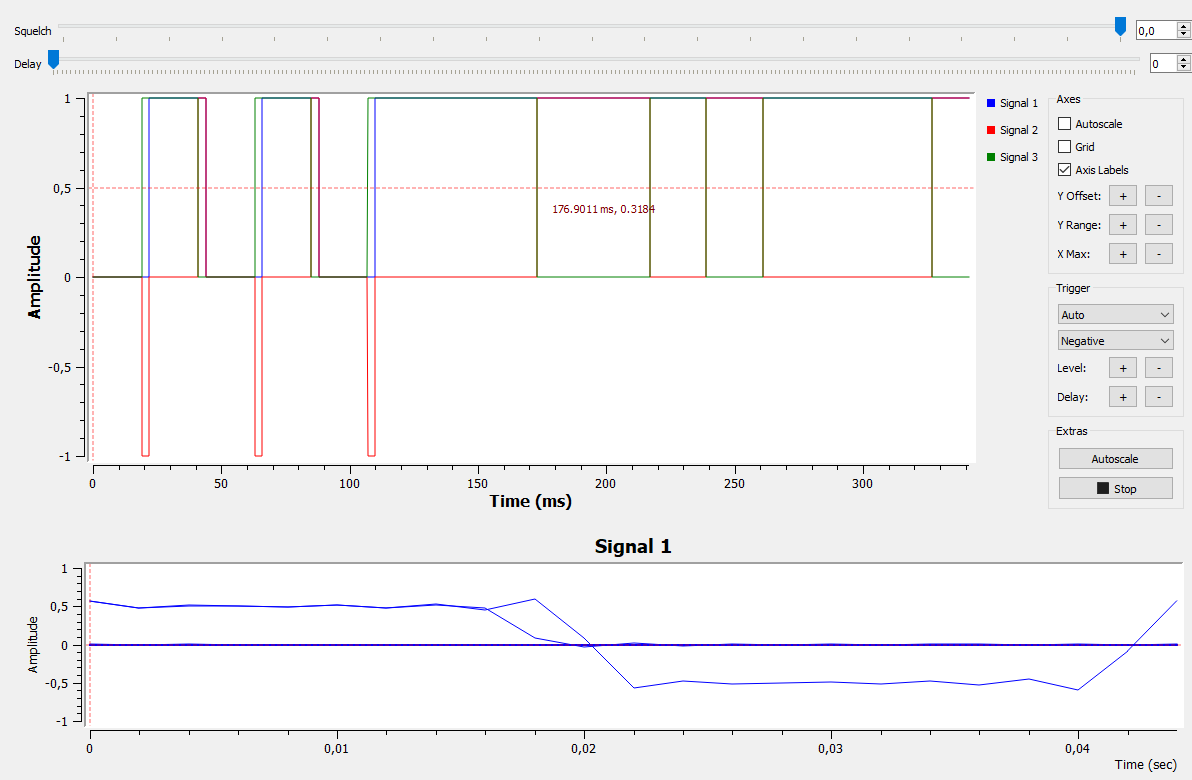
\includegraphics[scale=0.4]{fig/lab12/e1.png}
		\caption{Тестирование без шума и задержки}
		\label{pic:e1} % название для ссылок внутри кода
	\end{center}
\end{figure}

На графике есть 3 сигнала.
\begin{itemize}
    \item Синий сигнал - данные полученные приёмником. 
    \item Зелёный сигнал - данные переданные передатчиком.
    \item Красный сигнал - разница между двумя предыдущими. 
\end{itemize}

Если всё передаётся верно, то он д. б. равен нулю. Видим, что переднная и полученная информация разная. Дело в том, что всё блоки передатчика и приёмника не работают с бесконечно малой задержкой. Поэтому надо ввести задержку между приёмом и выдачей данных на диаграмму. Делается это при помощи блока Delay. Установил задержку 145.

    \begin{figure}[H]
	\begin{center}
		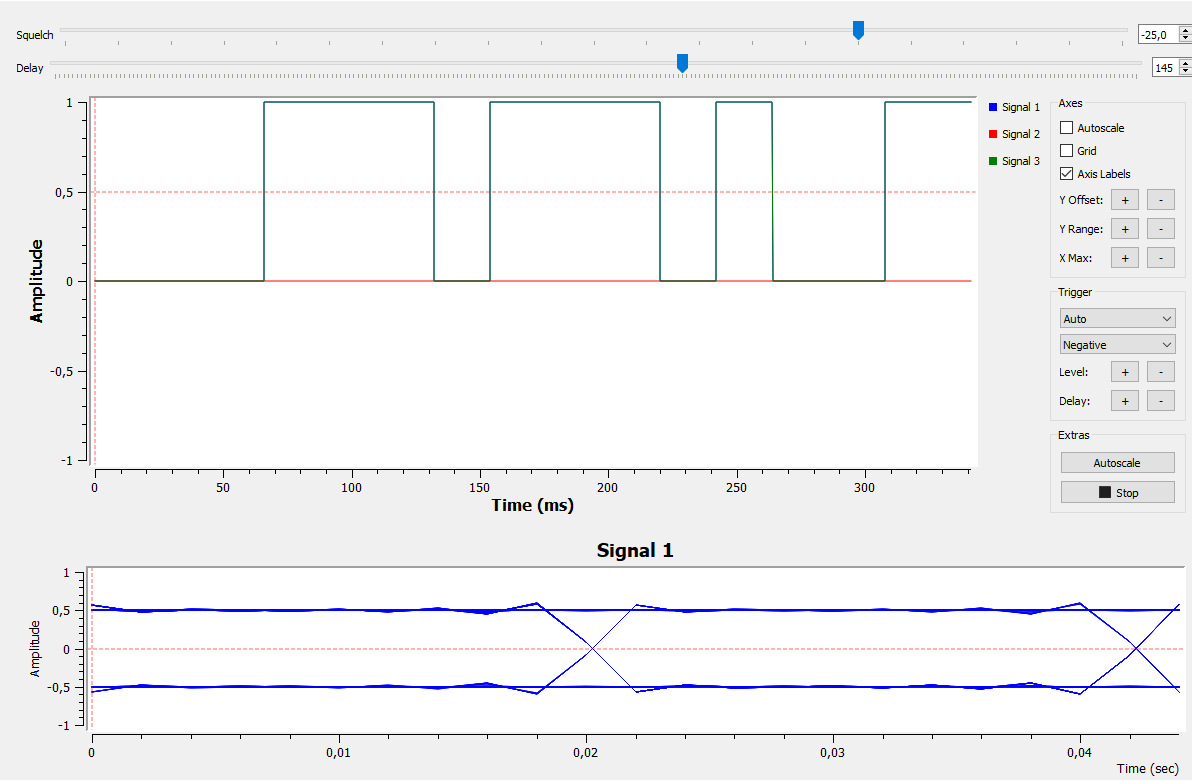
\includegraphics[scale=0.4]{fig/lab12/e2.png}
		\caption{Тестирование с нужной задержкой}
		\label{pic:e2} % название для ссылок внутри кода
	\end{center}
\end{figure}

На рисунке видно, что мы подверги сигнал шумам, но из-за фильтра это не помешало нам получить информацию.

\subsection{Вывод}
В данной работе был изучен новый способ модуляции. Как говорилось ранее, он довольно шумоустойчив из-за того, что информация передаётся при помощи изменений частоты, а не амплитуды. При помощи среды Radio GNU была создана модель и проверена на корректность.